\documentclass[main.tex]{subfiles}

\begin{document}

\section{Force Analysis}

\subsection{Vectors and Components}

A \gls{vector} is a quantity that has both magnitude and direction. Graphically a vector is an arrow used to represent quantities with both magnitude and direction. Two-dimensional vectors can be broken down into two components. A \gls{component} is a piece of a vector that points in either the vertical or the horizontal direction. The horizontal piece of a vector is known as the $x$-component. The vertical piece is the $y$-component. Components may be down graphically or mathematically, as shown in the following examples.

\begin{example}
    Find the $x$- and $y$-components of vector $A$ below.
\end{example}

\begin{center}
\def\Ax{6}
\def\Ay{4}
\begin{tikzpicture}
    \begin{axis}[width=8cm,height=8cm,
        axis lines = center,
        xlabel = $x$, 
        ylabel = $y$, 
        ymin=0, ymax=8,
        xmin=0, xmax=8,
        xtick={-8,-6,...,8},
        ytick={-8,-6,...,8},
        ymajorgrids=true,
        xmajorgrids=true,
        clip=false,
        ]
        \draw[ultra thick,->] (axis cs: 0,0) -- (\Ax,\Ay) node[above] {$\vec{A}$};
    \end{axis}
\end{tikzpicture}
\end{center}

\clearpage
\Solution The horizontal and vertical components, $A_x$ and $A_y$, respectively, are found graphically:

\begin{center}
\def\Ax{6}
\def\Ay{4}
\begin{tikzpicture}
    \begin{axis}[width=7cm,height=7cm,
        axis lines = center,
        xlabel = $x$, 
        ylabel = $y$, 
        ymin=0, ymax=8,
        xmin=0, xmax=8,
        xtick={-8,-6,...,8},
        ytick={-8,-6,...,8},
        ymajorgrids=true,
        xmajorgrids=true,
        clip=false,
        ]
        \draw[ultra thick,->] (axis cs: 0,0) -- (\Ax,\Ay) node[above] {$\vec{A}$};
        \draw[ultra thick,->,cyan] (0,0) -- (\Ax,0) node[above,pos=0.8] {$A_x = 6$};
        \draw[ultra thick,->,red] (\Ax,0) -- ++(0,\Ay) node[right,pos=0.9] {$A_y = 4$};
    \end{axis}
\end{tikzpicture}
\end{center}

Therefore, the $x$ and $y$ components of vector $A$ are

\begin{equation*}
    \vec{A}_x = 6 \quad \text{and} \quad \vec{A}_y = 4
\end{equation*}

\solutionEnd
\vspace{1em}

The $x$- and $y$-components are always perpendicular, or at \ang{90}, to each other. 

\begin{center}
    \pgfplotsset{compat=1.11}
    \def\A{6}
    \def\angle{55}
\begin{tikzpicture}
    \begin{axis}[width=6cm,height=6cm,
        axis lines=center,
        axis line style={black!20},
        xmin=0,xmax=5,
        ymin=0,ymax=5,
        clip=false,
        ticks=none,
        xlabel=$+x$,
        ylabel=$+y$,
    ]
    \draw[blue,thick,->] (0,0) -- ({\A*cos(\angle)},0) node[pos=0.5,below] {$\vec{A}_x$};
    \draw[red,thick,->] ({\A*cos(\angle)},0) -- ++(0,{\A*sin(\angle)}) node[pos=0.5, right] {$\vec{A}_y$};
    \draw[ultra thick,->] (0,0) -- ({\A*cos(\angle)},{\A*sin(\angle)}) node[pos=0.5,above left] {$\vec{A}$};
    \draw[thick] (0.6,0) arc (0:\angle:0.6) node[pos=0.75,right=2pt] {$\theta$};
    \end{axis}
\end{tikzpicture}
\captionsetup{type=figure,margin=1in,font=scriptsize}
\captionof{figure}{Vector $A$ and it's two components. $A_x$ is the horizontal component; $A_y$ is the vertical. The quantity $\theta$ is the angle between the $x$-axis and vector $A$.}
\label{xXmnIC}
\end{center}

Since they form a right triangle, they combine together to give the length of the overall vector in accordance with the Pythagorean Theorem:

\begin{equation} \label{NsyXHk}
    A^2 = A_x^2 + A_y^2
\end{equation}

\clearpage

\begin{example}
    Consider vector $A$, whose $x$- and $y$-components are 3 and 4, respectively. Calculate the magnitude of $\vec{A}$.
\end{example}

\begin{center}
\begin{tikzpicture}
    \begin{axis}[width=5cm,height=5cm,
        axis lines=center,
        axis line style={draw=none},
        xmin=0,xmax=4,
        ymin=0,ymax=4,
        clip=false,
        ticks=none,
    ]
    \draw[dashed,->] (0,0) -- (3,0) node[pos=0.5,below] {3};
    \draw[dashed,->] (3,0) -- ++(0,4) node[pos=0.5, right] {4};
    \draw[thick,->] (0,0) -- (3,4) node[pos=0.5,above left] {$\vec{A}$};
    \draw (0.6,0) arc (0:53.13:0.6);
    \end{axis}
\end{tikzpicture}
\end{center}

\Solution We are given the magnitudes of the horizontal and vertical components: $A_x = 3$ and $A_y = 4$. The unknown we are looking for is the magnitude of the resultant vector: $A =\ ?$

\vspace{1em}

The given and unknown quantities are related by the Pythagorean theorem, Equation \eqref{NsyXHk}, as

\begin{equation*}
    A^2 = A_x^2 + A_y^2
\end{equation*}

Substituting given values leads to 

\begin{equation*}
    A^2 = 3^2 + 4^2
\end{equation*}

which simplifies to

\begin{equation*}
    A^2 = 25
\end{equation*}

To solve for $A$, we take the square root of both sides:

\begin{equation*}
    \sqrt{A^2} = \sqrt{25}
\end{equation*}

Therefore, 

\begin{equation*}
    A = 5
\end{equation*}

The magnitude of the vector whose $x$- and $y$-components are 3 and 4 is 5. 

\solutionEnd

\begin{example}
    The magnitude of a two-dimensional vector is 185. If the magnitude of its vertical component is 153, calculate the magnitude of its $x$-component. 
\end{example}

\Solution We are given magnitudes of the vector and its $y$-component: $A = 185$ and $A_y = 153$. We are looking for the horizontal component: $A_x =\ ?$ The given and unknown quantities are related by the Pythagorean theorem (Eq.~\ref{NsyXHk}):

\begin{equation*}
    A^2 = A_x^2 + A_y^2
\end{equation*}

Substituting known values leads to 

\begin{equation*}
    185^2 = A_x^2 + 153^2
\end{equation*}

Since we are solving for $A_x$, let's re-write this equation by putting the unknown variable on the left, simply as 

\begin{equation*}
    A_x^2 + 153^2 = 185^2
\end{equation*}

We solve for the horizontal component as follows:

\begin{align*}
    \textbf{Add $153^2$} \qquad & A_x^2 + 153^2 \redminus \textcolor{red}{153^2} = 185^2 \redminus \textcolor{red}{153^2}\\[1ex]
    \textbf{Simplify} \qquad & A_x^2 = 185^2 - 153^2\\[1ex]
    \textbf{Simplify} \qquad & A_x^2 = \num{10816}\\[1ex]
    \textbf{Take square root} \qquad & \sqrt{A_x^2} = \sqrt{\num{10816}}\\[1ex]
    \textbf{Simplify} \qquad & A_x = 104
\end{align*}

Therefore, the magnitude of the horizontal ($x$) component of the vector is 104.

\solutionEnd

Take a look at Figure \ref{xXmnIC}. It's possible to find either the $x$- or $y$-component if you know both the magnitude of vector $A$ and the angle $\theta$. Vector $A$ and angle $\theta$ are related to the $x$- and $y$-components by the trig functions cosine (cos) and sine (sin), as follows:

\begin{align}
    A_x = A \cos{\theta} \label{06CyUc}\\[1ex]
    A_y = A \sin{\theta} \label{aBWDIc}
\end{align}

\begin{example}
    A vector with a magnitude of 25 is oriented \ang{36} above the horizontal, as shown below. Find the $x$- and $y$-components.
\end{example}

\begin{center}
\begin{tikzpicture}
    \begin{axis}[width=5cm,height=5cm,
        axis lines=center,
        axis line style={draw=none},
        xmin=0,xmax=4,
        ymin=0,ymax=4,
        clip=false,
        ticks=none,
    ]
    \draw[dashed,->] (0,0) -- ({5*cos(36)},0) node[pos=0.5,below] {$A_x$};
    \draw[dashed,->] ({5*cos(36)},0) -- ++(0,{5*sin(36)}) node[pos=0.5, right] {$A_y$};
    \draw[thick,->] (0,0) -- ({5*cos(36)},{5*sin(36)}) node[pos=0.5,above left] {25};
    \draw (0.6,0) arc (0:36:0.6) node [pos=0.75,right=2pt]{\ang{36}};
    \end{axis}
\end{tikzpicture}
\end{center}

\Solution We are given the vector's magnitude and angle: $A = 25$ and $\theta=\ang{36}$. By Equation~\eqref{06CyUc}, the horizontal component is

\begin{equation*}
    A_x = A \cos{\theta} = 25 \cos{(\ang{36})} = 20.2
\end{equation*}

The vertical component, by Equation \eqref{aBWDIc}, is

\begin{equation*}
    A_y = A \sin{\theta} = 25 \sin{(\ang{36})} = 14.7
\end{equation*}

\solutionEnd

\subsection{Free-body Diagrams} \label{SdNOfY}

A \gls{free-body diagram} shows all forces acting on an object. The object is a dot ($\bullet$) and the forces are vectors (arrows). When more than one force acts on an object, the \gls{net force} ($F_{\text{net}}$) is the sum of all forces. 

\begin{mdframed}[backgroundcolor=black!10]
\textit{Right Minus Left Rule}. In a free-body diagram, net force is rightward force(s) minus leftward force(s).

\begin{center}
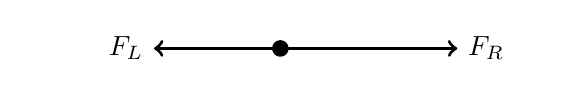
\begin{tikzpicture}
\pgfplotsset{compat=1.11}
    \begin{axis}[
        width=8cm, height=2cm,
        axis line style={draw=none},
        ticks=none,
        axis lines=middle,
        ymin=-1, ymax=1,
        xmin=-1, xmax=1,
        clip=false,
    ]
    \fill (0,0) circle (3pt);
    \draw[very thick,black,->] (0.05,0) -- (-0.5,0) node[left] {$F_{\text{L}}$};
    \draw[very thick,black,->] (-0.05,0) -- (+0.70,0) node[right] {$F_{\text{R}}$};
    % \node[right] at (1.3,0) {$F_{\text{net}} = F_{\text{R}} - F_{\text{L}}$};
    \end{axis}
\end{tikzpicture}
\end{center}
\vspace{-1em}

\begin{equation}
    \vec{F}_{\text{net}} = F_{\text{R}} - F_{\text{L}}
\end{equation}
\end{mdframed}

% Net force is calculated from a free-body diagram, as shown in the examples below. In a free-body diagram, the directions \textit{right} and \textit{up} are positive ($+$), and directions \textit{left} and \textit{down} are negative ($-$).

\begin{example} \label{ex:FnetFromFBD} 
    Two teams play tug-of-war. Team Red pushes right on a cart with a force of \SI{70}{newtons}. Team Blue applies a \SI{50}{N} leftward force. Draw a free-body diagram and calculate the net force on the cart.
\end{example}

\Solution

\begin{center}
    
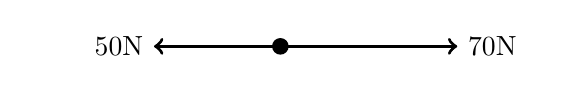
\begin{tikzpicture}
\pgfplotsset{compat=1.11}
\def\s{1}
    \begin{axis}[
        width=8cm, height=2cm,
        axis line style={draw=none},
        ticks=none,
        axis lines=middle,
        ymin=-\s, ymax=\s,
        xmin=-\s, xmax=\s,
        clip=false,
    ]
    \fill (0,0) circle (3pt);
    \draw[very thick,black,->] (0.05,0) -- (-0.5,0) node[left] {\SI{50}{N}};
    \draw[very thick,black,->] (-0.05,0) -- (+0.70,0) node[right] {\SI{70}{N}};
    \end{axis}
\end{tikzpicture}
\end{center}

Net force is rightward force \textit{minus} leftward force:

\begin{equation*}
    \vec{F}_{\text{net}} = 70 - 50 = +\SI{20}{N}\ .
\end{equation*}

Therefore, the \textit{net} force will be to the right with a magnitude of \SI{20}{N}.

\begin{example}
\href{https://youtu.be/7e3XhWMHolU}{Spongebob and Patrick} each apply a 50-newton rightward force on a treasure chest. Mr.~Krabs applies a \SI{75}{N} leftward force. (a) Draw a free-body diagram of the chest. (b) Calculate the net force on it.
\end{example}

\Solution (a) The free-body diagram is

\begin{center}
    
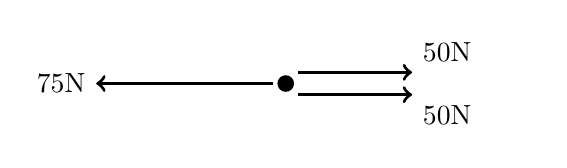
\begin{tikzpicture}
\pgfplotsset{compat=1.11}
\def\s{100} %scale
\def\FR{50} %rightward force
\def\FL{75} %leftward force
    \begin{axis}[
        width=8cm, height=3cm,
        axis line style={draw=none},
        ticks=none,
        axis lines=middle,
        ymin=-\s, ymax=\s,
        xmin=-\s, xmax=\s,
        clip=false,
    ]
    \fill (0,0) circle (3pt);
    \draw[very thick,black,->] (5,20) -- (\FR,20) node[above right] {\SI{\FR}{N}};
    \draw[very thick,black,->] (5,-20) -- (\FR,-20) node[below right] {\SI{\FR}{N}};
    \draw[very thick,black,->] (-5,0) -- (-\FL,0) node[left] {\SI{\FL}{N}};
    \end{axis}
\end{tikzpicture}
\end{center}

(b) Net force is the sum of all forces. Computing rightward minus leftward forces leads to
\vspace{-1em}

\begin{equation*}
    \vec{F}_{\text{net}} = 50 + 50 - 75 = +\SI{25}{N}\ .
\end{equation*}

\solutionEnd

\vspace{1em}

\subsection{Newton's Second Law of Motion} \label{kkBUgj}

\Gls{equilibrium} is the state when all forces on an object are balanced; the net force is zero ($\vec{F}_{\text{net}} = 0$), which implies that the object does not accelerate. A net force is also known as an unbalanced force. When a non-zero net force (e.g., $F_{\text{net}} = \SI{10}{N}$) acts on an object that's at rest, the object moves. More specifically, it accelerates: its velocity changes over a period of time.


\gls{NIIL} states that the net force on an object is equal to the mass of the object multiplied by its acceleration.

\begin{equation} \label{eq:NewtonIILaw} 
    F_{\mathrm{net}} = ma
\end{equation}

\begin{center}
    \begin{tabular}{cl|cl}
    \hline
    \textbf{Symbol} & \textbf{Quantity} & \textbf{SI Base Unit} & \textbf{Unit Symbol}  \\
    \hline\hline
    \rule{0pt}{2.5ex}
        $F_{\mathrm{net}}$ & net force & newton & N\\
        $m$ & mass & kilogram & kg\\
        $a$ & acceleration & meter per second squared & \SI{}{m/s^2}\\
    \hline
    \end{tabular}
\end{center}

According to Newton's 2nd Law, net force causes acceleration. When there is a net force on an object ($\vec{F}_{\text{net}} \neq 0$), the object will accelerate in the direction of the net force.


\begin{example} \label{ex:NetForce_Tony}
Tony pushes a 15-kg shopping cart and accelerates it by \SI{3.0}{m/s^2}. What is the net force Tony exerts on the cart?
\end{example}

\Solution We are given mass and acceleration: $m = \SI{15}{kg}$ and $a = \SI{3.0}{m/s^2}$. We want to find net force: $F_{\text{net}} =$ ? These three quantities are related by Newton's 2nd Law (Eq.~\ref{eq:NewtonIILaw}):

\begin{equation*}
    F_{\text{net}} = m a\ .
\end{equation*}

Substituting values leads to

\begin{equation*}
    F_{\text{net}} = (15)(3.0) = \SI{45}{N}.
\end{equation*}

Therefore, the net force is $\SI{45}{N}$. 

\solutionEnd

\begin{example} \label{ex:Solve_NIIL_a}
Santi pushes a lawn mower with a net force of \SI{51}{N}. The mass of the mower is \SI{24}{kg}. What is its acceleration?
\end{example}

\Solution We know net force and mass: $F_{\mathrm{net}} = \SI{51}{N}$ and $m = \SI{24}{kg}$. We want to find acceleration: $a =$ ? By Newton's 2nd Law,

\begin{equation*}
    F_{\mathrm{net}} = ma\ .
\end{equation*}

Substituting known values leads to,

\begin{equation*}
    51 = 24 a\ .
\end{equation*}

Solve this equation for acceleration by the following steps:

\begin{align*}
    \textbf{Write $a$ on left} \hspace{9cm} 
    & \hspace{-6cm} 24 a = 51\\[1ex]
    \textbf{Divide by 24} \hspace{9cm}
    & \hspace{-6cm} \frac{\cancel{24}a}{\textcolor{red}{\cancel{24}}} = \frac{51}{\textcolor{red}{24}}\\[1ex]
    \textbf{Simplify} \hspace{9cm}
    & \hspace{-6cm} a = 2.1
\end{align*}

Therefore, the acceleration of the lawn mower is  $a = \SI{2.1}{m/s^2}$.

\solutionEnd

\begin{example} \label{ex:TugOWar} 
Two teams play tug-of-war on a cart. One team pulls the cart leftward, and the other team pulls rightward. The net force and cart mass are shown in the free-body diagram below. What is the cart's acceleration?
\end{example}

\begin{center}
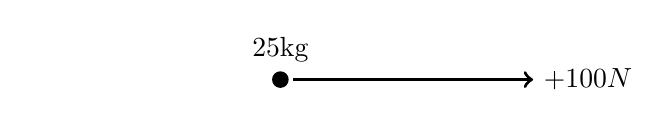
\begin{tikzpicture}
\pgfplotsset{compat=1.11}
\def\s{1}
    \begin{axis}[
        width=8cm, height=2cm,
        axis line style={draw=none},
        ticks=none,
        axis lines=middle,
        ymin=-\s, ymax=\s,
        xmin=-\s, xmax=\s,
        clip=false,
    ]
    \fill (0,0) circle (3pt) node[above=3pt] {\SI{25}{kg}};
    \draw[very thick,black,->] (0.05,0) -- (1,0) node[right] {$+\SI{100}{N}$};
    \end{axis}
\end{tikzpicture}
\end{center}



\Solution From the free-body diagram, we know that net force is $F_{\text{net}} = \SI{100}{N}$ and mass is $m = \SI{25}{kg}$. We want to find acceleration: $a =$ ?. Here, this example proceeds like Example~\ref{ex:Solve_NIIL_a}. Newton's second law is $F_{net} = ma$, and substituting values leads to

\begin{equation*}
    100 = 25 a\ .
\end{equation*}

Solving for acceleration, as we did in Example \ref{ex:Solve_NIIL_a}, leads to

\begin{equation*}
    a = \SI{4.0}{m/s^2}\ .
\end{equation*}

\vspace{2ex}

\cyanhrule


\subsection{Friction} \label{lk8L5k}

\Gls{friction} ($f$) is an external force that acts in a direction opposite to the object's velocity. Friction is present when surfaces touch, like when a cardboard box slides across a table.

\begin{example}
When Santi (from Example~\ref{ex:Solve_NIIL_a}) accelerates a 24-kg lawn mower, he's required to push against a force of friction from the grass. This frictional force has a magnitude of \SI{30}{N}. What is the force $F_a$ that Santi needs to apply on the mower to reach a net force of \SI{51}{N}?
\end{example}

\Solution Start by drawing a free-body diagram:

\begin{center}

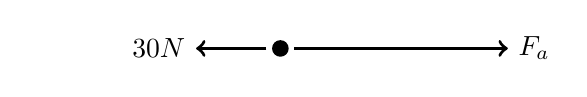
\begin{tikzpicture}
\pgfplotsset{compat=1.11}
\def\s{90}
    \begin{axis}[
        width=8cm, height=2cm,
        axis line style={draw=none},
        ticks=none,
        axis lines=middle,
        ymin=-\s, ymax=\s,
        xmin=-\s, xmax=\s,
        clip=false,
    ]
    \fill (0,0) circle (3pt);
    \draw[very thick,black,->] (5,0) -- (81,0) node[right] {$F_a$};
    \draw[very thick,black,->] (-5,0) -- (-30,0) node[left] {$\SI{30}{N}$};
    \end{axis}
\end{tikzpicture}
\end{center}

The desired net force is

\begin{equation*}
    F_{\text{net}} = \SI{51}{N}\ ,
\end{equation*}

but from the free-body diagram net force is

\begin{equation*}
    F_{\text{net}} = F_a - 30\ .
\end{equation*}

Equating these two expressions leads to

\begin{equation*}
    F_a - 30 = 51\ .
\end{equation*}

Solve for the applied force by adding 30 to both sides:

\begin{equation*}
    F_a - 30 \mathbin{\textcolor{red}{+}} \textcolor{red}{30} 
    = 51 \mathbin{\textcolor{red}{+}} \textcolor{red}{30} = 81\ .
\end{equation*}

Therefore, Santi's applied force is

\begin{equation*}
    F_a = \SI{81}{N}\ .
\end{equation*}

\begin{example} \label{ex:SilviaCouch} 
Silvia pushes a couch across the floor. Her applied force, the frictional force, and the couch's mass are shown in the free-body diagram below. (a) What is the net force on the couch? (b) If the mass of the couch is 20-kg, what is the acceleration? 
\end{example}
\vspace{-1em}

\begin{center}
    
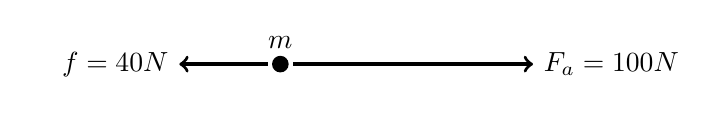
\begin{tikzpicture}
\pgfplotsset{compat=1.11}
\def\s{1}
    \begin{axis}[
        width=8cm, height=2cm,
        axis line style={draw=none},
        ticks=none,
        axis lines=middle,
        ymin=-\s, ymax=\s,
        xmin=-\s, xmax=\s,
        clip=false,
    ]
    \fill (0,0) circle (3pt) node[above=2pt] {$m$};
    \draw[very thick,black,->] (0.05,0) -- (1,0) node[right] {$F_a = \SI{100}{N}$};
    \draw[very thick,black,->] (-0.05,0) -- (-0.40,0) node[left] {$f = \SI{40}{N}$};
    \end{axis}
\end{tikzpicture}
\end{center}


\Solution (a) From the free-body diagram, net force is applied force \textit{minus} friction (or, right \textit{minus} left):

\begin{equation*}
    F_{\text{net}} = 100 - 40 = \SI{60}{N}\ .
\end{equation*}


(b) By Newton's 2nd Law, $F_{\text{net}} = m a$, or, in this case,

\begin{equation*}
    60 = 20 a\ .
\end{equation*}

Solving for acceleration (see Example \ref{ex:Solve_NIIL_a}) leads to

\begin{equation*}
    a = \SI{3.0}{m/s^2}\ .
\end{equation*}



\begin{example} \label{ex:StalledCar} 
A 2000-kg stalled car is pushed by two people. Assume each person applies an equal force. If the car accelerates at \SI{5.0}{m/s^2} against a frictional force of \SI{300}{N}, what is the force each person applies? 
\end{example}

\Solution Start by drawing a free body diagram:

\begin{center}
    
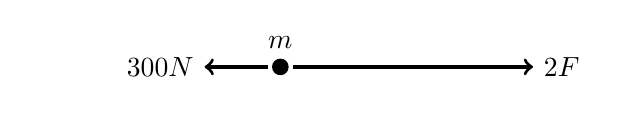
\begin{tikzpicture}
\pgfplotsset{compat=1.11}
\def\s{1}
    \begin{axis}[
        width=8cm, height=2cm,
        axis line style={draw=none},
        ticks=none,
        axis lines=middle,
        ymin=-\s, ymax=\s,
        xmin=-\s, xmax=\s,
        clip=false,
    ]
    \fill (0,0) circle (3pt) node[above=3pt] {$m$};
    \draw[very thick,black,->] (0.05,0) -- (1,0) node[right] {$2 F$};
    \draw[very thick,black,->] (-0.05,0) -- (-0.30,0) node[left] {$\SI{300}{N}$};
    \end{axis}
\end{tikzpicture}
\end{center}


We are given values of mass, acceleration, and friction: $m = \SI{2000}{kg}$, $a = \SI{5.0}{m/s^2}$, and $f = \SI{300}{N}$. The unknown is $F$, the force applied by each person. The net force on the car, by Newton's second law, is

\begin{equation*}
    F_{\text{net}} = ma = (2000)(5.0) = \SI{10000}{N}
\end{equation*}

But net force from the free-body diagram (right \textit{minus} left; see Example \ref{ex:FnetFromFBD}) is

\begin{equation*}
    F_{\text{net}} = 2F - 300
\end{equation*}

Since the two expressions above each represent net force, we can equate them as

\begin{equation*}
    2F - 300 = \SI{10000}{}
\end{equation*}

This equation is solved for $F$ as follows:

\begin{align*}
    \textbf{Add 300} \hspace{9cm} 
    & \hspace{-6cm} 2F - 300 \mathbin{\textcolor{red}{+}} \textcolor{red}{300} = \SI{10000}{} \mathbin{\textcolor{red}{+}} \textcolor{red}{300}\\[1ex]
    \textbf{Simplify} \hspace{9cm}
    & \hspace{-6cm} 2F = \SI{10300}{}\\[1ex]
    \textbf{Divide by 2} \hspace{9cm}
    & \hspace{-6cm} \frac{\cancel{2}F}{\textcolor{red}{\cancel{2}}} = \frac{\SI{10300}{}}{\textcolor{red}{2}}\\[1ex]
    \textbf{Simplify} \hspace{9cm} 
    & \hspace{-6cm} F = 5150
\end{align*}

Therefore, the force each person applies on the car is \SI{5150}{N}.

\solutionEnd

\vspace{1em}

\cyanhrule


\subsection{References \& Additional Resources}

\textit{YouTube}: ``Breaking Bad: Destroying the Evidence'' by \texttt{SonyPicturesDVD} (\href{https://youtu.be/gzCXowhks80?t=3}{click here}). An example of the magnetic force.

\textit{YouTube}: ``Jumping From Space! Red Bull Space Dive'' by \texttt{BBC Studios} (\href{https://youtu.be/E9oKEJ1pXPw}{click here}) An example of the gravitational force.

\textit{PhET Simulation}: ``Forces and Motion: Basics'' (\href{https://phet.colorado.edu/en/simulations/forces-and-motion-basics}{click here}).



\subsection{Exercises}



%%%%%%%%%%%

\begin{exercise} \label{RApeJt}
A leftward force of \SI{50}{N} and a rightward force of \SI{150}{N} are exerted on a cart. Draw a free body diagram. What is the net force?
\end{exercise}

\begin{exercise} \label{MUJe54}
A leftward force of \SI{200}{N} and a rightward force of \SI{150}{N} are exerted on a cart. What is the net force? 
\end{exercise}

\begin{exercise} \label{Uhrg0I}
A leftward force of \SI{200}{N} and a rightward force of \SI{200}{N} are exerted on a cart. What is the net force? 
\end{exercise}

\cyanhrule
\vspace{2ex}


\ref{Wu1JXi}--\ref{Js7KjP} Calculate the net force.

\begin{exercise} \label{Wu1JXi}
\phantom{.}
\vspace{-2em}
\end{exercise}

\begin{center}
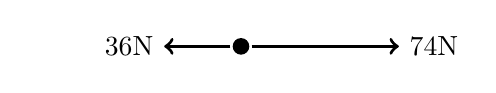
\begin{tikzpicture}
\pgfplotsset{compat=1.11}
\def\s{100} %scale
\def\FR{74} %rightward force
\def\FL{36} %leftward force
    \begin{axis}[
        width=7cm, height=2cm,
        axis line style={draw=none},
        ticks=none,
        axis lines=middle,
        ymin=-\s, ymax=\s,
        xmin=-\s, xmax=\s,
        clip=false,
    ]
    \fill (0,0) circle (3pt);
    \draw[very thick,black,->] (5,0) -- (\FR,0) node[right] {\SI{\FR}{N}};
    \draw[very thick,black,->] (-5,0) -- (-\FL,0) node[left] {\SI{\FL}{N}};
    \end{axis}
\end{tikzpicture}
\end{center}


\begin{exercise} \label{Tj5icu}
\phantom{.}
\vspace{-1cm}
\end{exercise}

\begin{center}
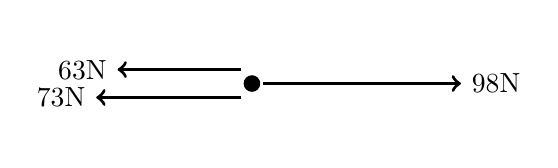
\begin{tikzpicture}
\pgfplotsset{compat=1.11}
\def\s{100} %scale
\def\FR{98} %rightward force
\def\FL{63} %leftward force
\def\FLL{73}
    \begin{axis}[
        width=7cm, height=3cm,
        axis line style={draw=none},
        ticks=none,
        axis lines=middle,
        ymin=-\s, ymax=\s,
        xmin=-\s, xmax=\s,
        clip=false,
    ]
    \fill (0,0) circle (3pt);
    \draw[very thick,black,->] (5,0) -- (\FR,0) node[right] {\SI{\FR}{N}};
    \draw[very thick,black,->] (-5,25) -- (-\FL,25) node[left] {\SI{\FL}{N}};
    \draw[very thick,black,->] (-5,-25) -- (-\FLL,-25) node[left] {\SI{\FLL}{N}};
    \end{axis}
\end{tikzpicture}
\end{center}

\begin{exercise} \label{nMwKjy}
\phantom{.}
\vspace{-3em}
\end{exercise}

\begin{center}
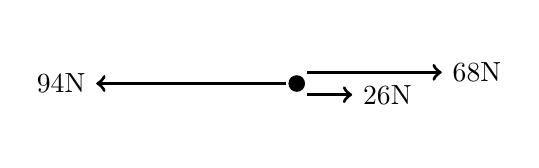
\begin{tikzpicture}
\pgfplotsset{compat=1.11}
\def\s{100} %scale
\def\FR{68} %rightward force
\def\FL{94} %leftward force
\def\FRR{26}
    \begin{axis}[
        width=7cm, height=3cm,
        axis line style={draw=none},
        ticks=none,
        axis lines=middle,
        ymin=-\s, ymax=\s,
        xmin=-\s, xmax=\s,
        clip=false,
    ]
    \fill (0,0) circle (3pt);
    \draw[very thick,black,->] (5,20) -- (\FR,20) node[right] {\SI{\FR}{N}};
    \draw[very thick,black,->] (5,-20) -- (\FRR,-20) node[right] {\SI{\FRR}{N}};
    \draw[very thick,black,->] (-5,0) -- (-\FL,0) node[left] {\SI{\FL}{N}};
    \end{axis}
\end{tikzpicture}
\end{center}


\begin{exercise} \label{Js7KjP}
\phantom{.}
\vspace{-3em}
\end{exercise}

\begin{center}
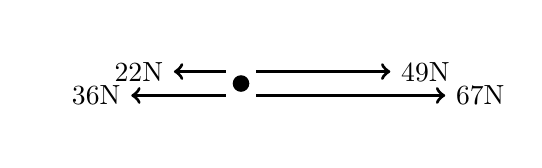
\begin{tikzpicture}
\pgfplotsset{compat=1.11}
\def\s{70} %scale
\def\FR{49} %rightward force
\def\FL{22} %leftward force
\def\FRR{67}
\def\FLL{36}
    \begin{axis}[
        width=7cm, height=3cm,
        axis line style={draw=none},
        ticks=none,
        axis lines=middle,
        ymin=-\s, ymax=\s,
        xmin=-\s, xmax=\s,
        clip=false,
    ]
    \fill (0,0) circle (3pt);
    \draw[very thick,black,->] (5,15) -- (\FR,15) node[right] {\SI{\FR}{N}};
    \draw[very thick,black,->] (5,-15) -- (\FRR,-15) node[right] {\SI{\FRR}{N}};
    \draw[very thick,black,->] (-5,15) -- (-\FL,15) node[left] {\SI{\FL}{N}};
    \draw[very thick,black,->] (-5,-15) -- (-\FLL,-15) node[left] {\SI{\FLL}{N}};
    \end{axis}
\end{tikzpicture}
\end{center}

%%%%%%%%%%%

\begin{exercise} \label{01Hh51}
What is the unit of force? What is the unit symbol?
\end{exercise}

\begin{exercise} \label{YQwD8z}
One newton (N) is approximately the force on your hand from the weight of an apple. Newton's 2nd Law suggests that the newton may be equivalently expressed in terms of a the kilogram, the meter, and the second.  Using Eq.~(\ref{eq:NewtonIILaw}) to guide you, write \SI{1}{N} in terms of kg, m, and s. (\textit{Hint}: Replace the quantity symbols with their unit symbols.)
\end{exercise}

\begin{exercise} \label{aBCVA3}
Antonio pushes a 12-kg shopping cart and accelerates it by \SI{2.0}{m/s^2}. Draw the free-body diagram on the cart. What is the net force Antonio exerts on the cart?
\end{exercise}

\begin{exercise} \label{Sm9Zw6}
    If a 10-kg object accelerates at \SI{5.2}{m/s^2}, what is the net force exerted on it? Include a free-body diagram.  
\end{exercise}

\begin{exercise} \label{RbjKEg}
    A 63.0-kg sprinter starts a race with an acceleration of \SI{4.20}{m/s^2}. What is the net force on him?
\end{exercise}

\begin{exercise} \label{goj4oA}
    A cleaner pushes a 4.50-kg laundry cart with a net force of \SI{60.0}{N}. Calculate the cart's acceleration.
\end{exercise}

\begin{exercise} \label{G333de}
    The net force on a 68-kg filing cabinet is \SI{240}{N}. What is the cabinet's acceleration?
\end{exercise}

\begin{exercise} \label{8M4KDp}
    7800 newtons of net force are applied by the engine on a car to accelerate the vehicle at \SI{2.4}{m/s^2}. What is the mass of the car?
\end{exercise}

\begin{exercise} \label{EAtsO8}
    When a net force of \SI{84}{N} are exerted on an object, the object accelerates at \SI{7.0}{m/s^2}. What is the object's mass?
\end{exercise}

\begin{exercise} \label{vuAqX8}
    Solve Newton's Second Law ($F_{\text{net}} = ma$) for acceleration using no numbers, only variables. \textit{Hint}: Follow Example~\ref{ex:Solve_NIIL_a}.
\end{exercise}

\begin{exercise} \label{zVvXad}
    Solve Newton's 2nd Law for mass $m$ using only variables, no numbers.
\end{exercise}

\begin{exercise} \label{XfTcUv}
Team Red pushes a cart with a rightward force of \SI{184}{N}. Team blue pushes it with a \SI{122}{N} force to the left. The cart's mass is \SI{15.5}{kg}. (a) Draw the free-body diagram. (b) What is the cart's acceleration?
\end{exercise}

\begin{exercise} \label{uawqLb}
    Two horizontal forces on a \SI{2.0}{kg} box are \SI{13}{N} and \SI{-19}{N}. (a) Draw the free-body diagram of the box. (b) Calculate the acceleration of the box. 
\end{exercise}

\begin{exercise} \label{FWDsH3}
The object represented by the free-body diagram below accelerates at \SI{-4.0}{m/s^2}. Find the mass $m$ of the object.
\end{exercise}

\begin{center}
    
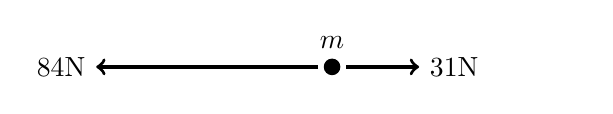
\begin{tikzpicture}
\pgfplotsset{compat=1.11}
\def\s{90}
    \begin{axis}[
        width=8cm, height=2cm,
        axis line style={draw=none},
        ticks=none,
        axis lines=middle,
        ymin=-\s, ymax=\s,
        xmin=-\s, xmax=\s,
        clip=false,
    ]
    \fill (0,0) circle (3pt) node[above=3pt] {$m$};
    \draw[very thick,black,->] (5,0) -- (31,0) node[right] {\SI{31}{N}};
    \draw[very thick,black,->] (-5,0) -- (-84,0) node[left] {\SI{84}{N}};
    \end{axis}
\end{tikzpicture}
\end{center}


\begin{exercise} \label{GeuEOb}
What is the acceleration of the object in the free-body diagram below?
\end{exercise}

\begin{center}

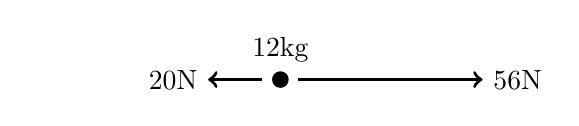
\begin{tikzpicture}
\pgfplotsset{compat=1.11}
\def\s{70}
    \begin{axis}[
        width=8cm, height=2cm,
        axis line style={draw=none},
        ticks=none,
        axis lines=middle,
        ymin=-\s, ymax=\s,
        xmin=-\s, xmax=\s,
        clip=false,
    ]
    \fill (0,0) circle (3pt) node[above=3pt]{\SI{12}{kg}};
    \draw[very thick,black,->] (5,0) -- (56,0) node[right] {\SI{56}{N}};
    \draw[very thick,black,->] (-5,0) -- (-20,0) node[left] {\SI{20}{N}};
    \end{axis}
\end{tikzpicture}
\end{center}


\begin{exercise} \label{zaZxeE}
When horizontal forces \SI{69}{N} and \SI{-42}{N} act on a wagon, it accelerates at \SI{3.0}{m/s^2}. (a) Draw the free-body diagram. (b) What is the mass of the wagon?
\end{exercise}

\begin{exercise} \label{ejRkLz}
The external forces applied when pushing a table across the floor are shown in the free-body diagram below. (a) What is the net force on the table? (b) If the table's mass is \SI{30}{kg}, what is its acceleration? 
\end{exercise}
\vspace{-2em}

\begin{center}
\begin{tikzpicture}
\pgfplotsset{compat=1.11}
\def\s{60}
    \begin{axis}[
        width=8cm, height=4cm,
        axis line style={draw=none},
        ticks=none,
        axis lines=middle,
        ymin=-\s, ymax=\s,
        xmin=-\s, xmax=\s,
        clip=false,
    ]
    \fill (0,0) circle (3pt);
    \draw[very thick,black,->] (5,0) -- (49,0) node[right] {$F_a = \SI{49}{N}$};
    \draw[very thick,black,->] (-5,0) -- (-25,0) node[left] {$f = \SI{25}{N}$};
    \end{axis}
\end{tikzpicture}
\end{center}

%%%%%%%%%

\begin{exercise} \label{lqMcA5}
The net force on a shopping cart is \SI{76}{N}. The person pushing the cart pushes against a frictional force of \SI{12}{N}. (a) Draw the free-body diagram showing the frictional and applied forces. (b) What is the person's applied force?
\end{exercise}

\begin{exercise} \label{Og290b}
The net force on an object is $\vec{F}_{\text{net}} = \SI{-25}{N}$. If the applied force is \SI{-46}{N}, what is the frictional force? 
\end{exercise}

\begin{center}
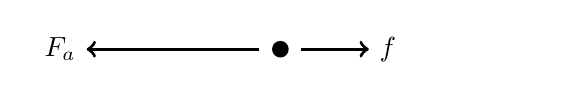
\begin{tikzpicture}
\pgfplotsset{compat=1.11}
\def\s{60}
    \begin{axis}[
        width=8cm, height=2cm,
        axis line style={draw=none},
        ticks=none,
        axis lines=middle,
        ymin=-\s, ymax=\s,
        xmin=-\s, xmax=\s,
        clip=false,
    ]
    \fill (0,0) circle (3pt);
    \draw[very thick,black,->] (5,0) -- (21,0) node[right] {$f$};
    \draw[very thick,black,->] (-5,0) -- (-46,0) node[left] {$F_a$};
    \end{axis}
\end{tikzpicture}
\end{center}

\begin{exercise} \label{naDHpo}
A 1965-kg stalled car is pushed by two people. Assume each person applies an equal force. If the car accelerates at \SI{3.5}{m/s^2} against a frictional force of \SI{480}{N}, what is the force each person applies? 
\end{exercise}

\begin{exercise} \label{w6N0j0}
14 people push an 8100-kg bus to get it started. An acceleration of at least \SI{7.0}{m/s^2} is required to start the bus, and friction between the bus and the road is \SI{900}{N}. Assuming each individual applies the same force, what is the magnitude of this individual force?
\end{exercise}

\begin{exercise} \label{WHMhQG}
    What is the answer to Example~\ref{ex:StalledCar} if there were five people pushing instead of two? Assume each person applies the same force and all other things being equal.
\end{exercise}

\begin{exercise} \label{DV094w}
Four \href{https://en.wikipedia.org/wiki/Spacecraft_propulsion#/media/File:Shuttle_Main_Engine_Test_Firing.jpg}{thrusters} propel a 2100-kg jet forward though the atmosphere against \SI{650}{N} of air resistance. If the jet accelerates at \SI{49}{m/s^2}, what is the force applied be each thruster? 
\end{exercise}

\begin{exercise} \label{e1ANRE}
Solve Example \ref{ex:StalledCar} for $F$ generally (without any numbers) using only the variables $f$, $m$, $a$, and $n$, where $n$ is the number of equal forces exerted on the object.
\end{exercise}




\begin{exercise}
Calculate the net force from the free-body diagram below.


\begin{center}
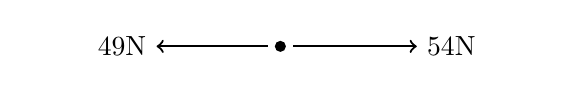
\begin{tikzpicture}
\pgfplotsset{compat=1.11}
\begin{axis}[
    width=8cm,height=2cm,
    axis line style={draw=none},
    ticks=none,
    xmin=-10,xmax=10,
    ymin=-10,ymax=10,
    clip=false,
]
    \fill (0,0) circle (2pt);
    \draw[thick,->] (0.5,0) -- (5.4,0) node[right] {\SI{54}{N}};
    \draw[thick,->] (-0.5,0) -- (-4.9,0) node[left] {\SI{49}{N}};
\end{axis}  
\end{tikzpicture}
\end{center}
\end{exercise}

\begin{exercise}
The sprinter Jessica, whose mass is 41.0-kg, starts a race with an acceleration of \SI{3.93}{m/s^2}. What is the net force on her?


{\color{red} Answer: \SI{161}{N}}

\end{exercise}

\begin{exercise}
If a net force of \SI{21000}{N} is exerted on a 750-kg vehicle, what is the vehicle's acceleration?

{\color{red} Answer: \SI{28}{m/s^2}}

\end{exercise}

\begin{exercise}
    The net force on an object accelerating at \SI{8.0}{m/s^2} is \SI{256}{N}. What is the object's mass?

    {\color{red} Ans: \SI{32}{kg}}

\end{exercise}


\subsection{Glossary}

\printnoidxglossaries

\clearpage

\subsection{Answers to Select Exercises}

\begin{multicols}{2}
\ref{WTFwXI}. (a) No, because the cart will not stay in motion if it is acted on by a net force. (b) A net force supplied by friction between the floor and wheels.\\
\ref{MB3Xar} (a) Since the bear has more mass, it has more inertia. (b) The bear will have a greater tendency than you to stay in motion \textit{in a straight line}; it's less able to do zig-zag motions.\\
\ref{RApeJt}. $+\SI{100}{N}$\\
\ref{MUJe54}. $-\SI{50}{N}$\\
\ref{Uhrg0I}. \SI{0}{N}\\
\ref{Wu1JXi}. $+\SI{38}{N}$\\
\ref{Tj5icu}. $-\SI{38}{N}$\\
\ref{nMwKjy}. \SI{0}{N}\\
\ref{Js7KjP}. $+\SI{58}{N}$\\
\ref{01Hh51}. newton (N)\\
\ref{YQwD8z}. $\SI{1}{N} \equiv \SI{1}{kg} \cdot \SI{1}{m/s^2}$\\
\ref{aBCVA3}. \SI{24}{N}\\
\ref{Sm9Zw6}. \SI{52}{N}\\
\ref{RbjKEg}. \SI{265}{N}\\
\ref{goj4oA}. \SI{13.3}{m/s^2}\\
\ref{G333de}. \SI{3.53}{m/s^2}\\
\ref{8M4KDp}. \SI{3250}{kg}\\
\ref{EAtsO8}. \SI{12}{kg}\\
\ref{vuAqX8}. $a = \frac{F_{\text{net}}}{m}$\\
\ref{zVvXad}. $m = \frac{F_{\text{net}}}{a}$\\
\ref{XfTcUv}. (b) \SI{4.0}{m/s^2}\\
\ref{uawqLb}. \SI{-3.0}{m/s^2}\\
\ref{FWDsH3}. \SI{13}{kg}\\
\ref{GeuEOb}. \SI{3.0}{m/s^2}\\
\ref{zaZxeE}. \SI{9.0}{kg}\\
\ref{ejRkLz}. \SI{0.8}{m/s^2}\\
\ref{lqMcA5}. \SI{64}{N}\\
\ref{Og290b}. $+\SI{21}{N}$\\
\ref{naDHpo}. \SI{3679}{N}\\
\ref{w6N0j0}. \SI{4114}{N}\\
\ref{WHMhQG}. \SI{2060}{N}\\
\ref{DV094w}. \SI{25888}{N}\\
\ref{e1ANRE}. $F = \frac{ma + f}{n}$\\





\end{multicols}

\end{document}